% elementos pré-textuais 

% título do sumário
\ifdefined\contentsname
  \renewcommand*\contentsname{SUMÁRIO}
\else
  \newcommand\contentsname{SUMÁRIO}
\fi

% capa 
\imprimircapa

% folha de rosto 
% o * indica que haverá a ficha bibliográfica 
\imprimirfolhaderosto*

% ficha catalográfica 
%\begin{fichacatalografica}
%    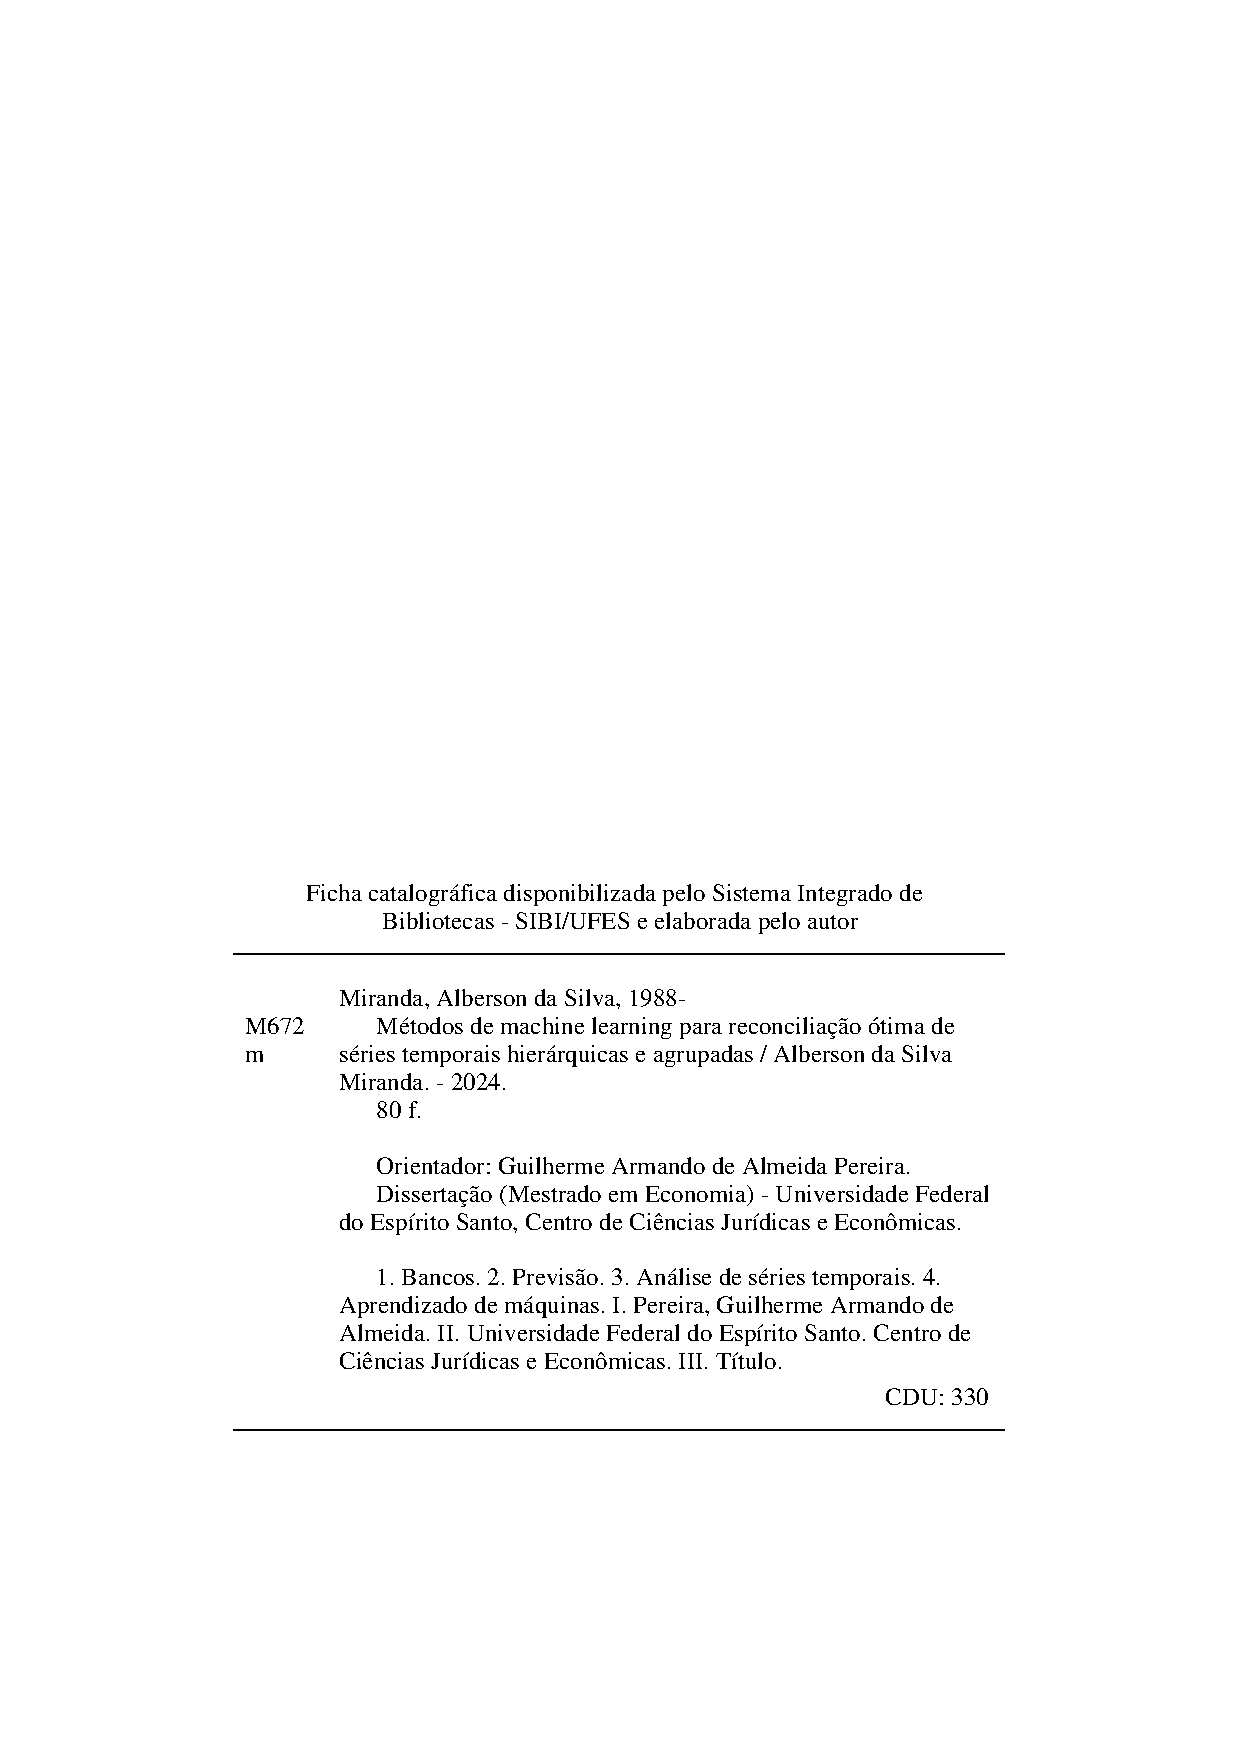
\includepdf{ficha_ufes.pdf}
%\end{fichacatalografica}


% substituir pela ficha em pdf fornecida pela UFES após defesa 
\begin{fichacatalografica}
	\sffamily
	\vspace*{\fill}					% Posição vertical
	\begin{center}					% Minipage Centralizado
	\fbox{\begin{minipage}[c][8cm]{15cm}		% Largura
	\small
	\imprimirautor
	
	\hspace{0.5cm} \imprimirtitulo  / \imprimirautor. --
	\imprimirlocal, \imprimirdata-
	
	\hspace{0.5cm} \thelastpage p. : il. (algumas color.) ; 30 cm.\\
	
	\hspace{0.5cm} \imprimirorientadorRotulo~\imprimirorientador\\
	
	\hspace{0.5cm}
	\parbox[t]{\textwidth}{\imprimirtipotrabalho~--~\imprimirinstituicao,
	\imprimirdata.}\\
	
	\hspace{0.5cm}
		1. Palavra-chave1.
		2. Palavra-chave2.
		2. Palavra-chave3.
		I. Orientador.
		II. Universidade xxx.
		III. Faculdade de xxx.
		IV. Título 			
	\end{minipage}}
	\end{center}
\end{fichacatalografica}

% folha de aprovação 
%
%\begin{folhadeaprovacao}
%    \includepdf{folhadeaprovacao_final.pdf}
%\end{folhadeaprovacao}


% substituir pela folha assinada pela banca após defesa 
\begin{folhadeaprovacao}

  \begin{center}
    {\ABNTEXchapterfont\large\imprimirautor}

    \vspace*{\fill}\vspace*{\fill}
    \begin{center}
      \ABNTEXchapterfont\bfseries\Large\imprimirtitulo
    \end{center}
    \vspace*{\fill}
    
    \hspace{.45\textwidth}
    \begin{minipage}{.5\textwidth}
        \imprimirpreambulo
        \vspace*{1cm}
        Aprovada em xx de xx de 20xx.\\[2cm]
        \textbf{COMISSÃO EXAMINADORA} \\
        \assinatura{\textbf{\imprimirorientador} \\ Universidade Federal do Espírito Santo \\ Orientador} 
        \assinatura{\textbf{Professor} \\ Instituição}
        \assinatura{\textbf{Professor} \\ Instituição}
        %\assinatura{\textbf{Professor} \\ Convidado 3}
        %\assinatura{\textbf{Professor} \\ Convidado 4}
    \end{minipage}%
   \end{center}
  
\end{folhadeaprovacao}

%% dedicatória 
%\begin{dedicatoria}
%   \vspace*{\fill}
%   \centering
%   \noindent
%   \textit{Exemplo de dedicatória,\\\lipsum[10].} \vspace*{\fill}
%\end{dedicatoria}

%% agradecimentos 
%\begin{agradecimentos}
%\lipsum[30]
%
%\lipsum[30]
%
%\end{agradecimentos}

% epígrafe 
%\begin{epigrafe}
%    \vspace*{\fill}
%	\begin{flushright}
%		\textit{``Modelo de epígrafe, \\
%		modelo de epígrafe.''}
%	\end{flushright}
%\end{epigrafe}

% resumo 

\setlength{\absparsep}{18pt}
\begin{resumo}
  \lipsum[30]

  \textbf{Palavras-chave}: palavra-chave1. palavra-chave2. palavra-chave3.
\end{resumo}

% abstract 
\begin{resumo}[Abstract]
  \begin{otherlanguage*}{english}
    \lipsum[30]

    \vspace{\onelineskip}
 
    \noindent 
    \textbf{Keywords}: keyword1. keyword2. keyword3.
  \end{otherlanguage*}
\end{resumo}

% lista de ilustrações 
\pdfbookmark[0]{\listfigurename}{lof}
\listoffigures*
\cleardoublepage

% lista de quadros 
\pdfbookmark[0]{\listofquadrosname}{loq}
\listofquadros*
\cleardoublepage

% lista de tabelas 
\pdfbookmark[0]{\listtablename}{lot}
\listoftables*
\cleardoublepage

% lista de abreviaturas 
\begin{siglas}
  \item[MinT] \textit{Minimum Trace}
  \item[MCRL] Modelo Clássico de Regressão Linear
  \item[MQO] Mínimos Quadrados Ordinários
  \item[MQP] Mínimos Quadrados Ponderados
\end{siglas}

% lista de símbolos 
\begin{simbolos}
  \item[$ t $] Tempo dentro da amostra
  \item[$ T $] Último tempo dentro da amostra, quantidade de observações numa série
  \item[$ h $] Horizonte de previsão, tempo fora da amostra
  \item[$ \Omega $] Conjunto de dados dentro da amostra
  \item[$ y $] Série temporal dentro da amostra
  \item[$ \hat{y} $] Série temporal estimada
  \item[$ \tilde{y} $] Série temporal reconciliada
  \item[$ n $] Número de séries na hierarquia
  \item[$ m $] Número de séries no menor nível da hierarquia
  \item[$ k $] Número de níveis na hierarquia
  \item[$ \mathbfit{S} $] Matriz de soma
  \item[$ \mathbfit{G} $] Matriz de reconciliação
  \item[$\{...\}$] Conjunto
  \item[$|\{...\}|$] Número de elementos em um conjunto
\end{simbolos}

% sumário 
\pdfbookmark[0]{\contentsname}{toc}
\tableofcontents*
\cleardoublepage

% elementos textuais 
\textual